\documentclass[11pt]{article}
\usepackage{reusv}
\graphicspath{{figures/}}

\setborderthickness{0.5pt}
\setbordermargin{1cm}
\setbordercolor{black}

\begin{document}
\drawborder
\thispagestyle{firstpage}

%% ============================================================
%%  TITLE BLOCK
%% ============================================================
\slimtitle{수치 검증: 비공면 전이와 경로 제약}
\lightertitle{수치 검증 업데이트:\\
비공면 궤도 전이와 경로 제약 검증}

{\normalsize\textit{Research Note No.~014 $|$ bezier-orbit-transfer-scp}}\par\medskip

\def\lighterdate{March 29, 2026}
\lighterauthor{Suwon Lee$^{\dagger}$}

\lighteraddress{$^\dagger$}{Future Mobility Control Lab, Kookmin University, Seoul, Korea}
\lighteremail{suwon.lee@kookmin.ac.kr}

%% ============================================================
%%  ABSTRACT
%% ============================================================
\begin{abstract}
\cite{report008}에서는 공면 궤도전이 시나리오 V1--V3으로
베지어--SCP 프레임워크의 기본 동작을 검증하였다.
본 노트에서는 검증 범위를 \textbf{비공면 3차원 궤도전이}
(경사각, RAAN 변경)와 \textbf{경로 제약}(궤도 반경 하한)으로 확장한다.
4개 시나리오 V4--V7을 제시하며,
경사각 변경(V4), 이심률+경사각 동시 변경(V5),
RAAN 변경+경로 제약(V6), SOCP+비공면+경로 제약(V7)을 다룬다.
전 시나리오에서 SCP 수렴을 확인하였으며,
경계조건 위반은 $O(10^{-4})$ 수준이다.
경로 제약은 \cite{report013}의 드 카스텔조 세분화 기반으로 구현되었다.
\end{abstract}

%% ============================================================
\section{검증 체계 확장}
%% ============================================================

\cite{report008}의 검증 시나리오 V1--V3은 모두 공면($i=0$) 궤도전이였다.
이후 추가된 기능을 반영하여 검증 범위를 확장한다:
\begin{itemize}
  \item \textbf{비공면 전이}: 경사각($i$), 승교점 적경($\Omega$) 변경
  \item \textbf{경로 제약}: 궤도 반경 하한 $r_{\min}$ (\cite{report013})
  \item \textbf{결합 테스트}: SOCP 추력 제약 + 비공면 + 경로 제약 동시 적용
\end{itemize}

모든 시나리오는 정규화 단위~\cite{report001}로 수행하며,
$N=12$, 섭동 레벨~0 (J2), RK4 드리프트 ($n_{\mathrm{steps}}=200$)를 사용한다.
Table~\ref{tab:scenarios}에 시나리오 개요를 정리하였다.

\begin{table}[h]
\centering
\caption{검증 시나리오 V4--V7 설정.}
\label{tab:scenarios}
\begin{tabular}{llllll}
\toprule
ID & 초기 궤도 & 종말 궤도 & $t_f^*$ & 제약 & 유형 \\
\midrule
V4 & $a{=}1, e{=}0, i{=}0^\circ$ & $a{=}1, e{=}0, i{=}28.5^\circ$ & 4.0 & QP & 경사각 \\
V5 & $a{=}1, e{=}0, i{=}15^\circ$ & $a{=}1.3, e{=}0.3, i{=}15^\circ$ & 5.0 & QP & 이심률+고도 \\
V6 & $a{=}1, e{=}0.01, i{=}10^\circ$ & $a{=}1.2, e{=}0.01, i{=}30^\circ, \Omega{=}20^\circ$ & 5.0 & QP+$r_{\min}$ & RAAN+경로 \\
V7 & $a{=}1, e{=}0, i{=}0^\circ$ & $a{=}1.2, e{=}0, i{=}20^\circ$ & 5.0 & SOCP+$r_{\min}$ & 통합 \\
\bottomrule
\end{tabular}
\end{table}

%% ============================================================
\section{V4: 경사각 변경}
%% ============================================================

\subsection{시나리오 설정}

LEO 원형궤도에서 경사각만 $0^\circ \to 28.5^\circ$로 변경하는 순수 면외 전이이다.
반장축과 이심률은 유지하며, 진근점이각 $\nu_f = \pi$이다.
추력 제약 없이 QP 모드로 풀었다.

\subsection{결과}

SCP는 33회 반복 후 수렴하였다.
경계조건 위반은 $4.26 \times 10^{-4}$로 허용치 $10^{-3}$ 이내이다.
최적 비용 $J^* = 0.2427$, $\Delta V^* = 1.39$이다.

이 시나리오에서 RK4 적분 스텝 수의 영향이 크게 나타났다.
$n_{\mathrm{steps}} = 50$에서는 BC 위반이 $4 \times 10^{-3}$에서 정체하여
미수렴하였으나, $n_{\mathrm{steps}} = 200$으로 증가시키면
BC 위반이 $4 \times 10^{-4}$까지 감소하여 수렴하였다.
비공면 전이에서는 $z$축 운동이 추가되어
드리프트 적분의 정밀도 요구가 높아지기 때문이다.

Fig.~\ref{fig:v4_3d}에 3차원 전이 궤적을,
Fig.~\ref{fig:v4_profiles}에 상태변수 및 추력 프로파일을 나타내었다.
면외($z$축) 성분의 비영(非零) 추력이 경사각 변경을 수행한다.

\begin{figure}[htbp]
\centering
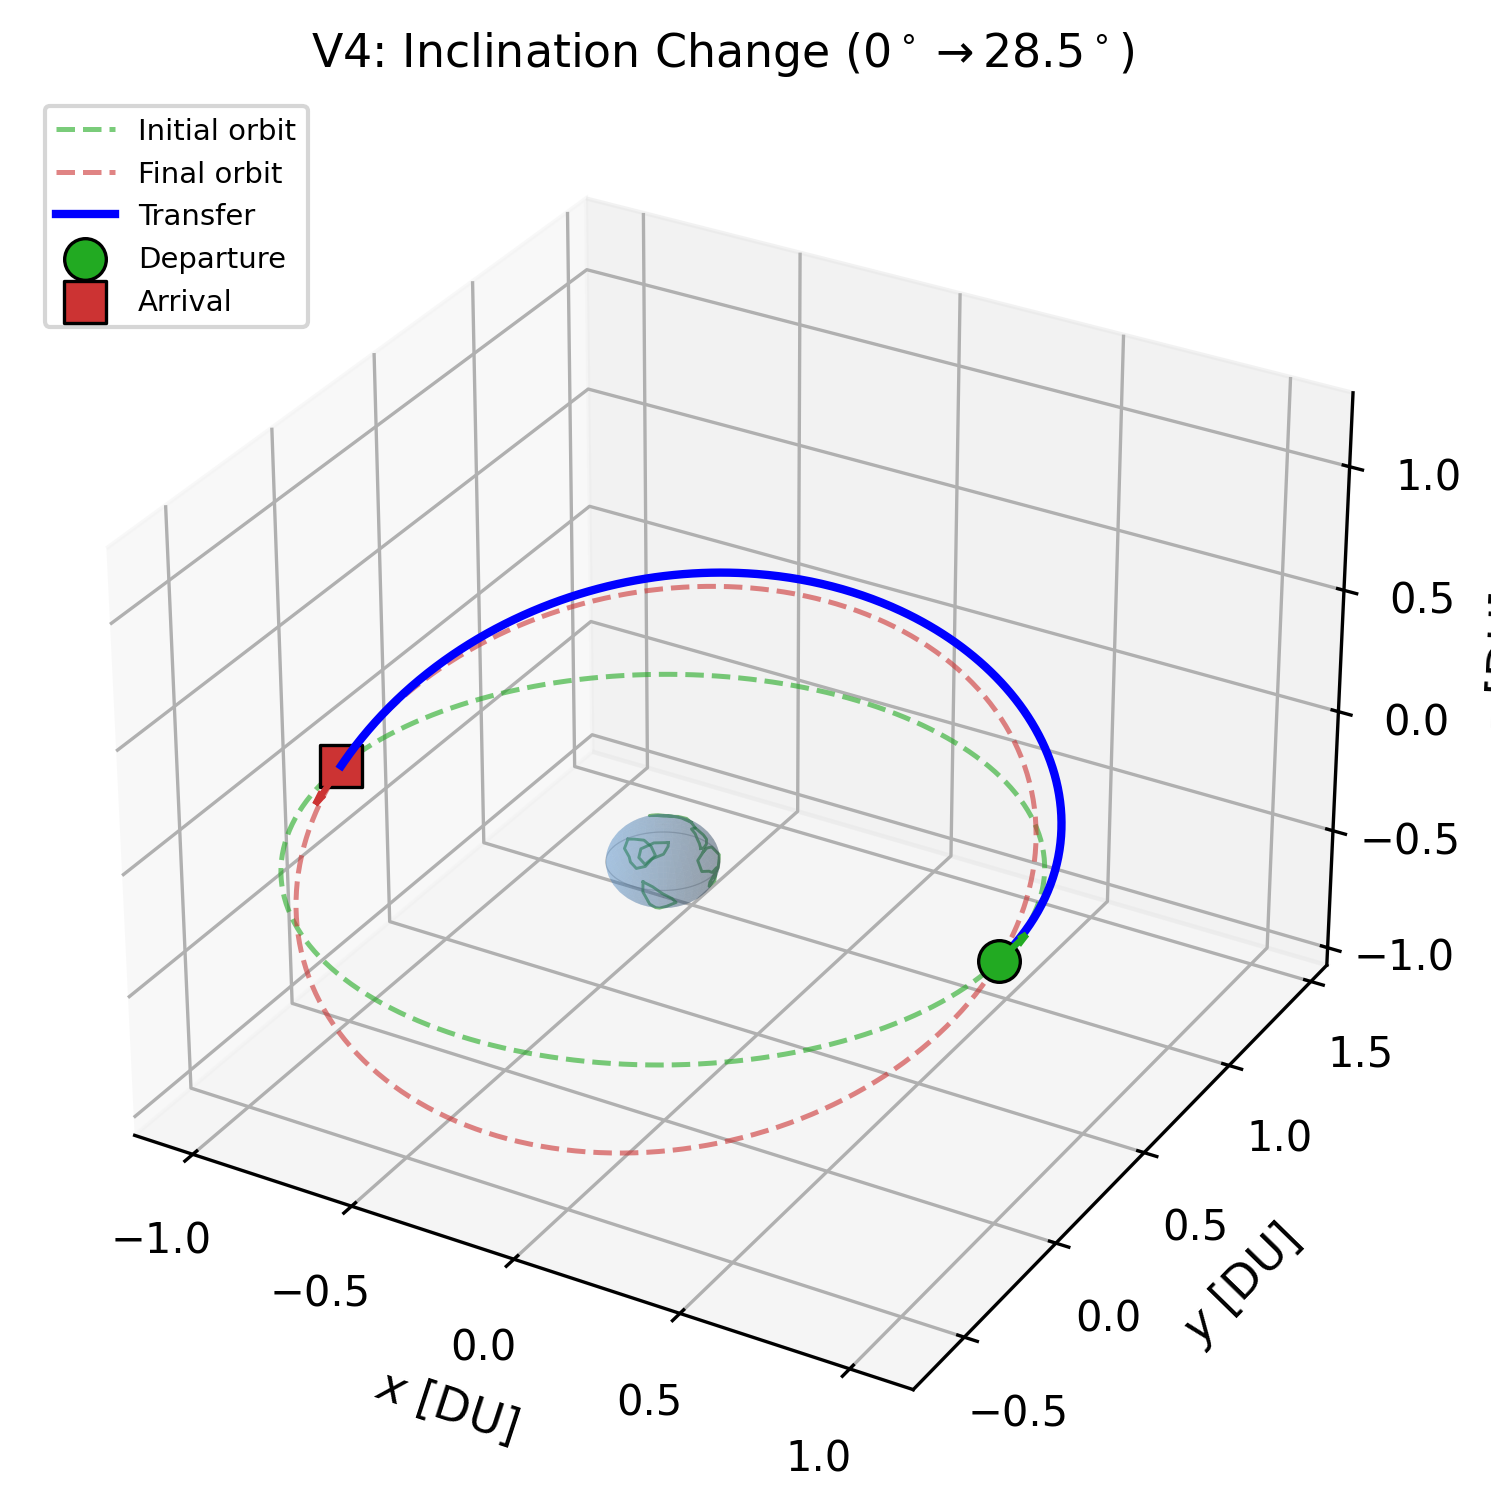
\includegraphics[width=0.75\linewidth]{v4_3d.png}
\caption{V4: 경사각 변경 ($i$: $0^\circ \to 28.5^\circ$) 3차원 전이 궤적.
         녹색 점선은 초기 궤도면, 적색 점선은 종말 궤도면을 나타낸다.}
\label{fig:v4_3d}
\end{figure}

\begin{figure}[htbp]
\centering
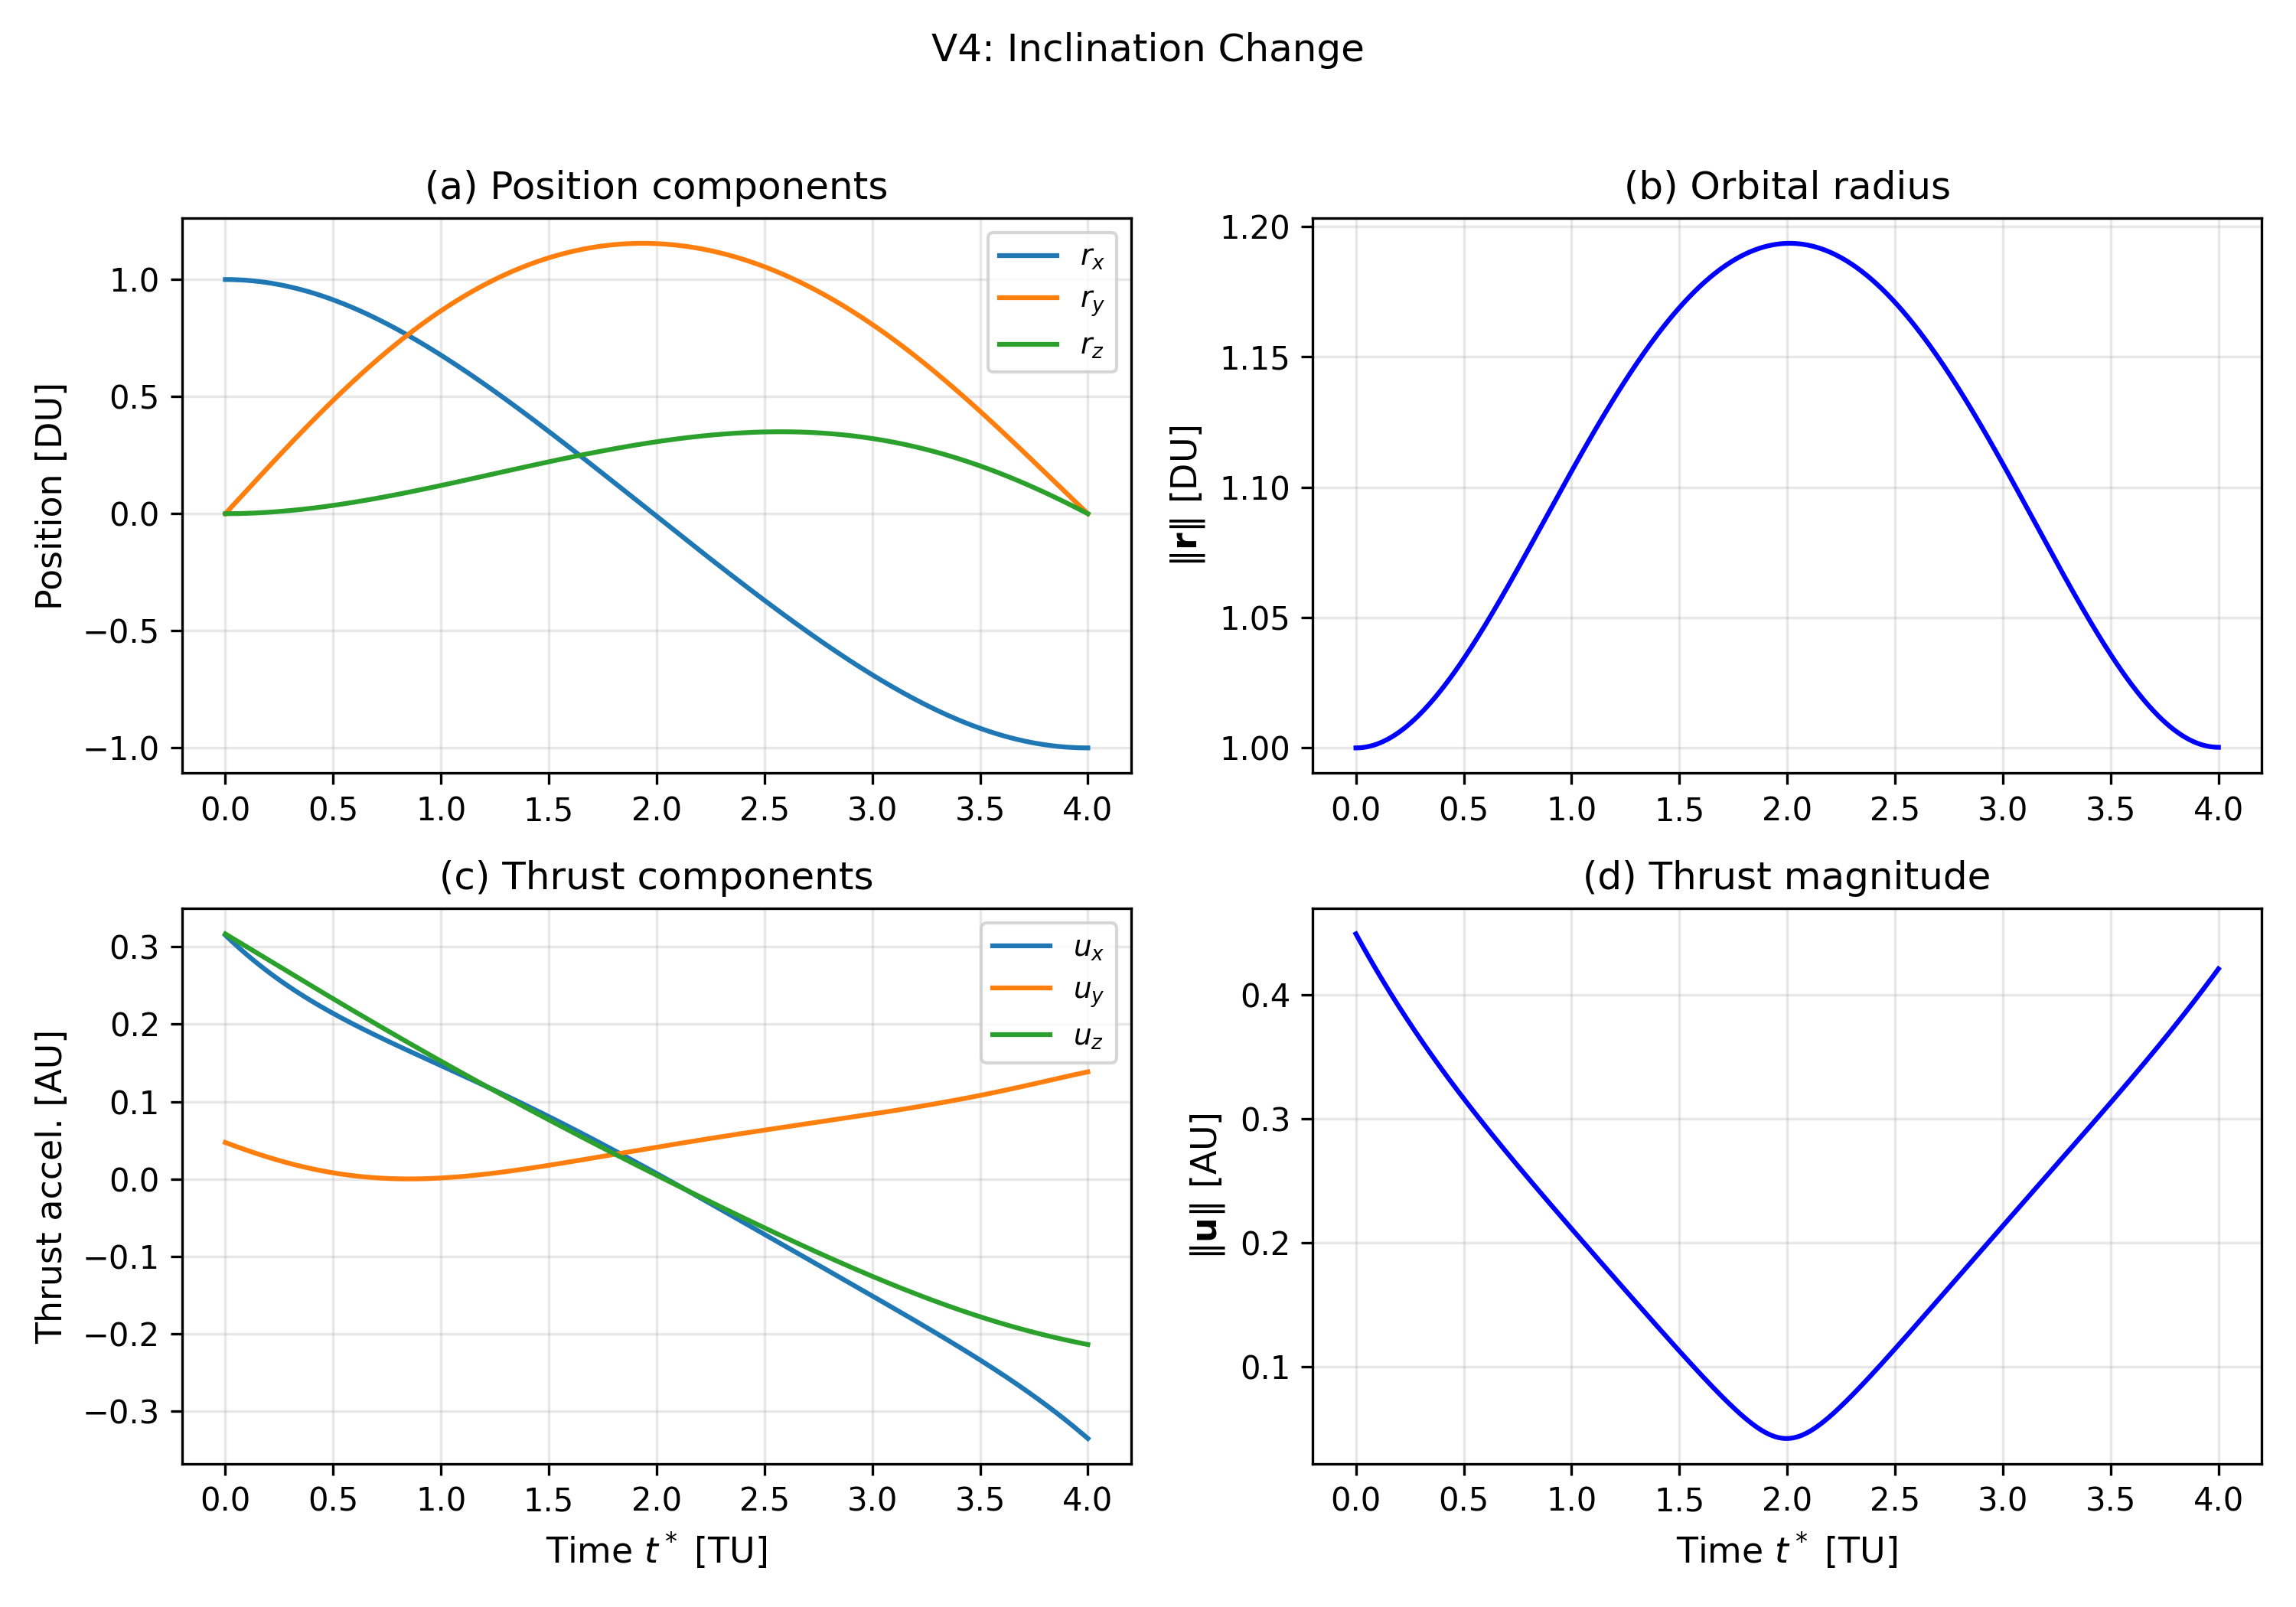
\includegraphics[width=\linewidth]{v4_profiles.png}
\caption{V4: 위치 성분 (a), 궤도 반경 (b), 추력 성분 (c), 추력 크기 (d).}
\label{fig:v4_profiles}
\end{figure}

%% ============================================================
\section{V5: 고도+이심률+경사각 동시 변경}
%% ============================================================

\subsection{시나리오 설정}

경사각 $i=15^\circ$를 유지하면서 반장축을 $1.0 \to 1.3$,
이심률을 $0 \to 0.3$으로 변경하고 근점인수를 $90^\circ$로 회전한다.
궤도 모양과 크기가 동시에 바뀌는 복합 전이이다.

\subsection{결과}

33회 반복 후 수렴, BC 위반 $5.40 \times 10^{-4}$,
$J^* = 0.0864$, $\Delta V^* = 0.93$이다.
이심률 변경으로 추력 프로파일이 비대칭적으로 나타나며,
근점 부근에서 추력이 집중되는 특성을 보인다.
Fig.~\ref{fig:v5_3d}에 3차원 궤적을,
Fig.~\ref{fig:v5_profiles}에 상태변수 프로파일을 나타내었다.
초기 원형궤도(녹색)에서 종말 타원궤도(파란색)로의 크기 변화가 명확하다.

\begin{figure}[htbp]
\centering
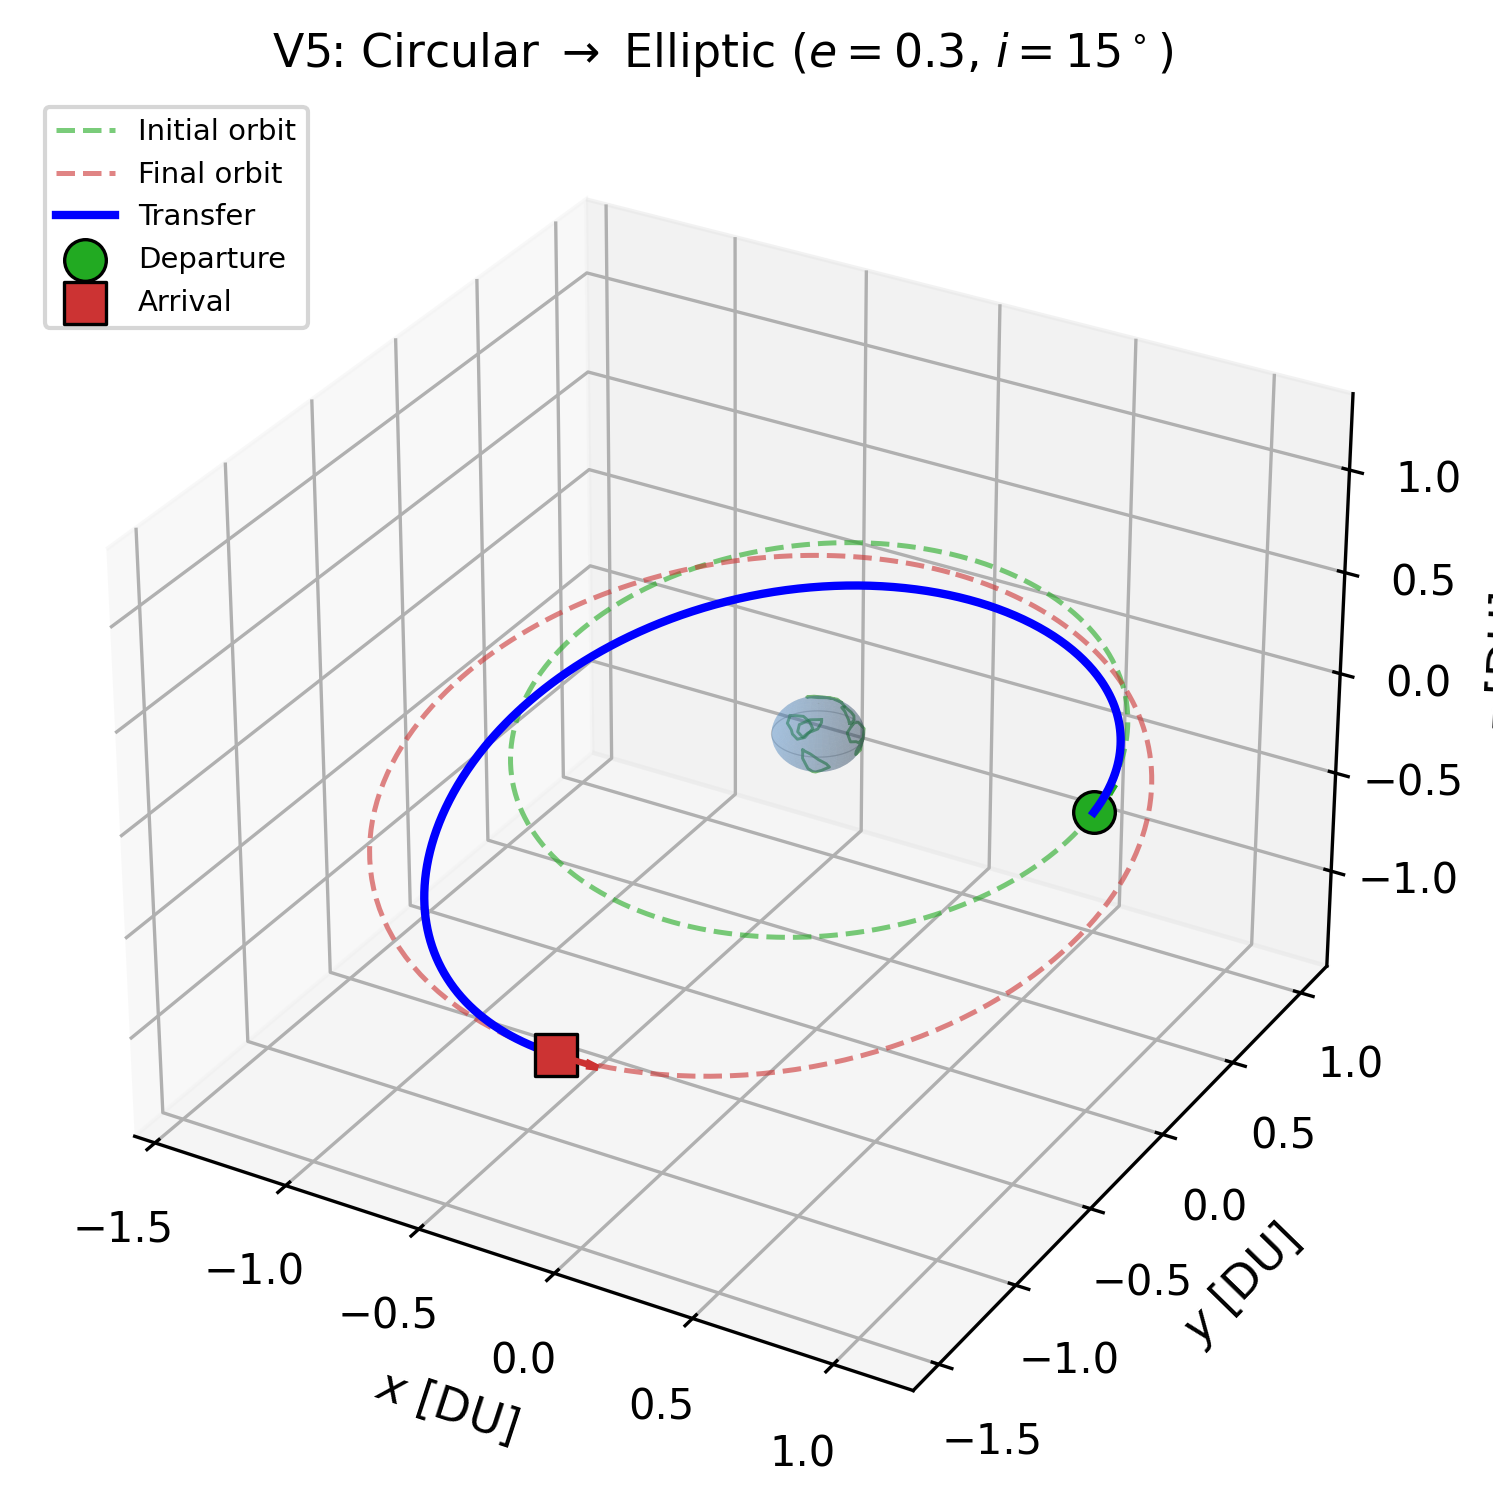
\includegraphics[width=0.75\linewidth]{v5_3d.png}
\caption{V5: 원형$\to$타원($e{=}0.3$, $i{=}15^\circ$) 3차원 전이 궤적.}
\label{fig:v5_3d}
\end{figure}

\begin{figure}[htbp]
\centering
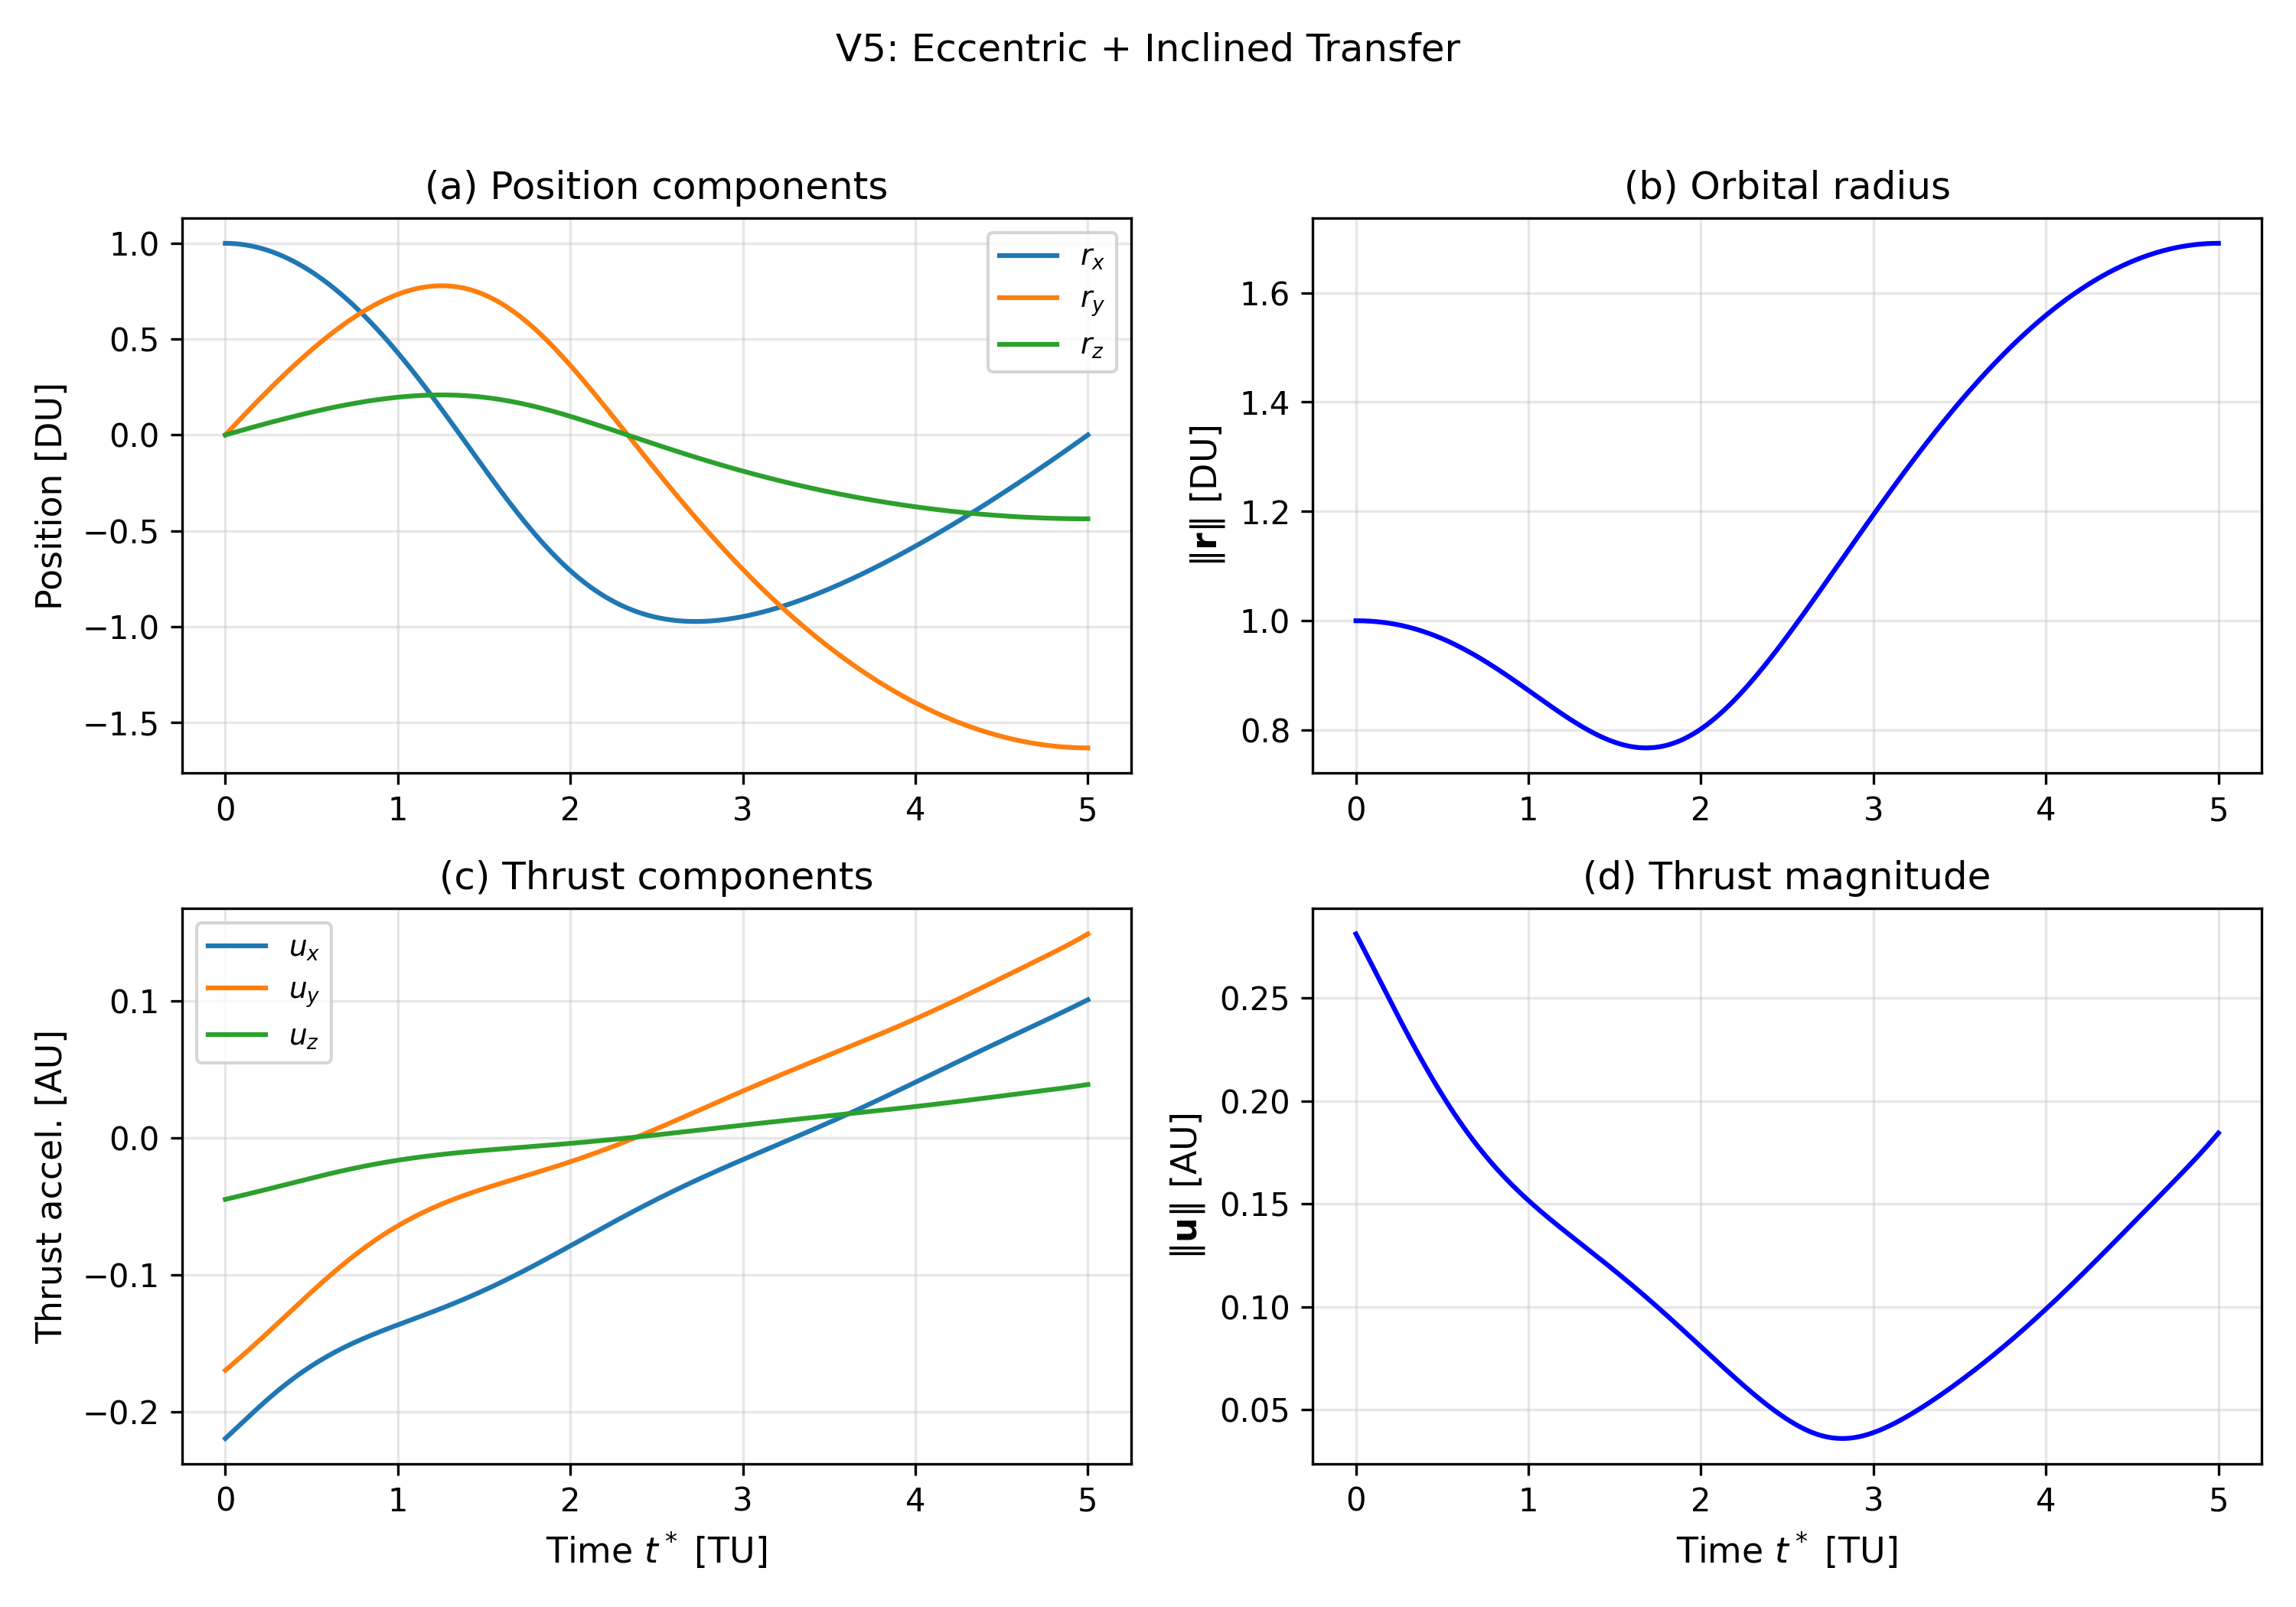
\includegraphics[width=\linewidth]{v5_profiles.png}
\caption{V5: 위치 성분 (a), 궤도 반경 (b), 추력 성분 (c), 추력 크기 (d).}
\label{fig:v5_profiles}
\end{figure}

%% ============================================================
\section{V6: RAAN 변경 + 경로 제약}
%% ============================================================

\subsection{시나리오 설정}

경사각 $10^\circ \to 30^\circ$, RAAN $0^\circ \to 20^\circ$를 동시 변경하며,
반장축을 $1.0 \to 1.2$로 키운다.
궤도 반경 하한 $r_{\min} = 0.9$를 경로 제약으로 부과한다.
드 카스텔조 세분화 $K=8$을 사용하여
$K \times (N{+}3) = 120$개의 부등식 제약이 추가된다.

\subsection{결과}

37회 반복 후 수렴, BC 위반 $5.28 \times 10^{-4}$,
$J^* = 0.1218$, $\Delta V^* = 1.10$이다.

경로 제약의 효과를 분석하면:
제약 없는 경우의 궤적 반경 최솟값은 $0.990$으로,
$r_{\min} = 0.9$보다 이미 크다.
따라서 이 시나리오에서 경로 제약은 \textbf{비활성}(inactive)이며,
비용 차이는 사실상 없다 ($< 0.01\%$).
이는 경로 제약이 필요 없는 궤적에 대해 솔버가 올바르게 동작함을 확인한 것이다.
Fig.~\ref{fig:v6_3d}에 3차원 궤적을,
Fig.~\ref{fig:v6_profiles}에 상태 프로파일을 나타내었다.
초기 궤도면(녹색)과 종말 궤도면(파란색)의 경사 차이가 드러난다.

\begin{figure}[htbp]
\centering
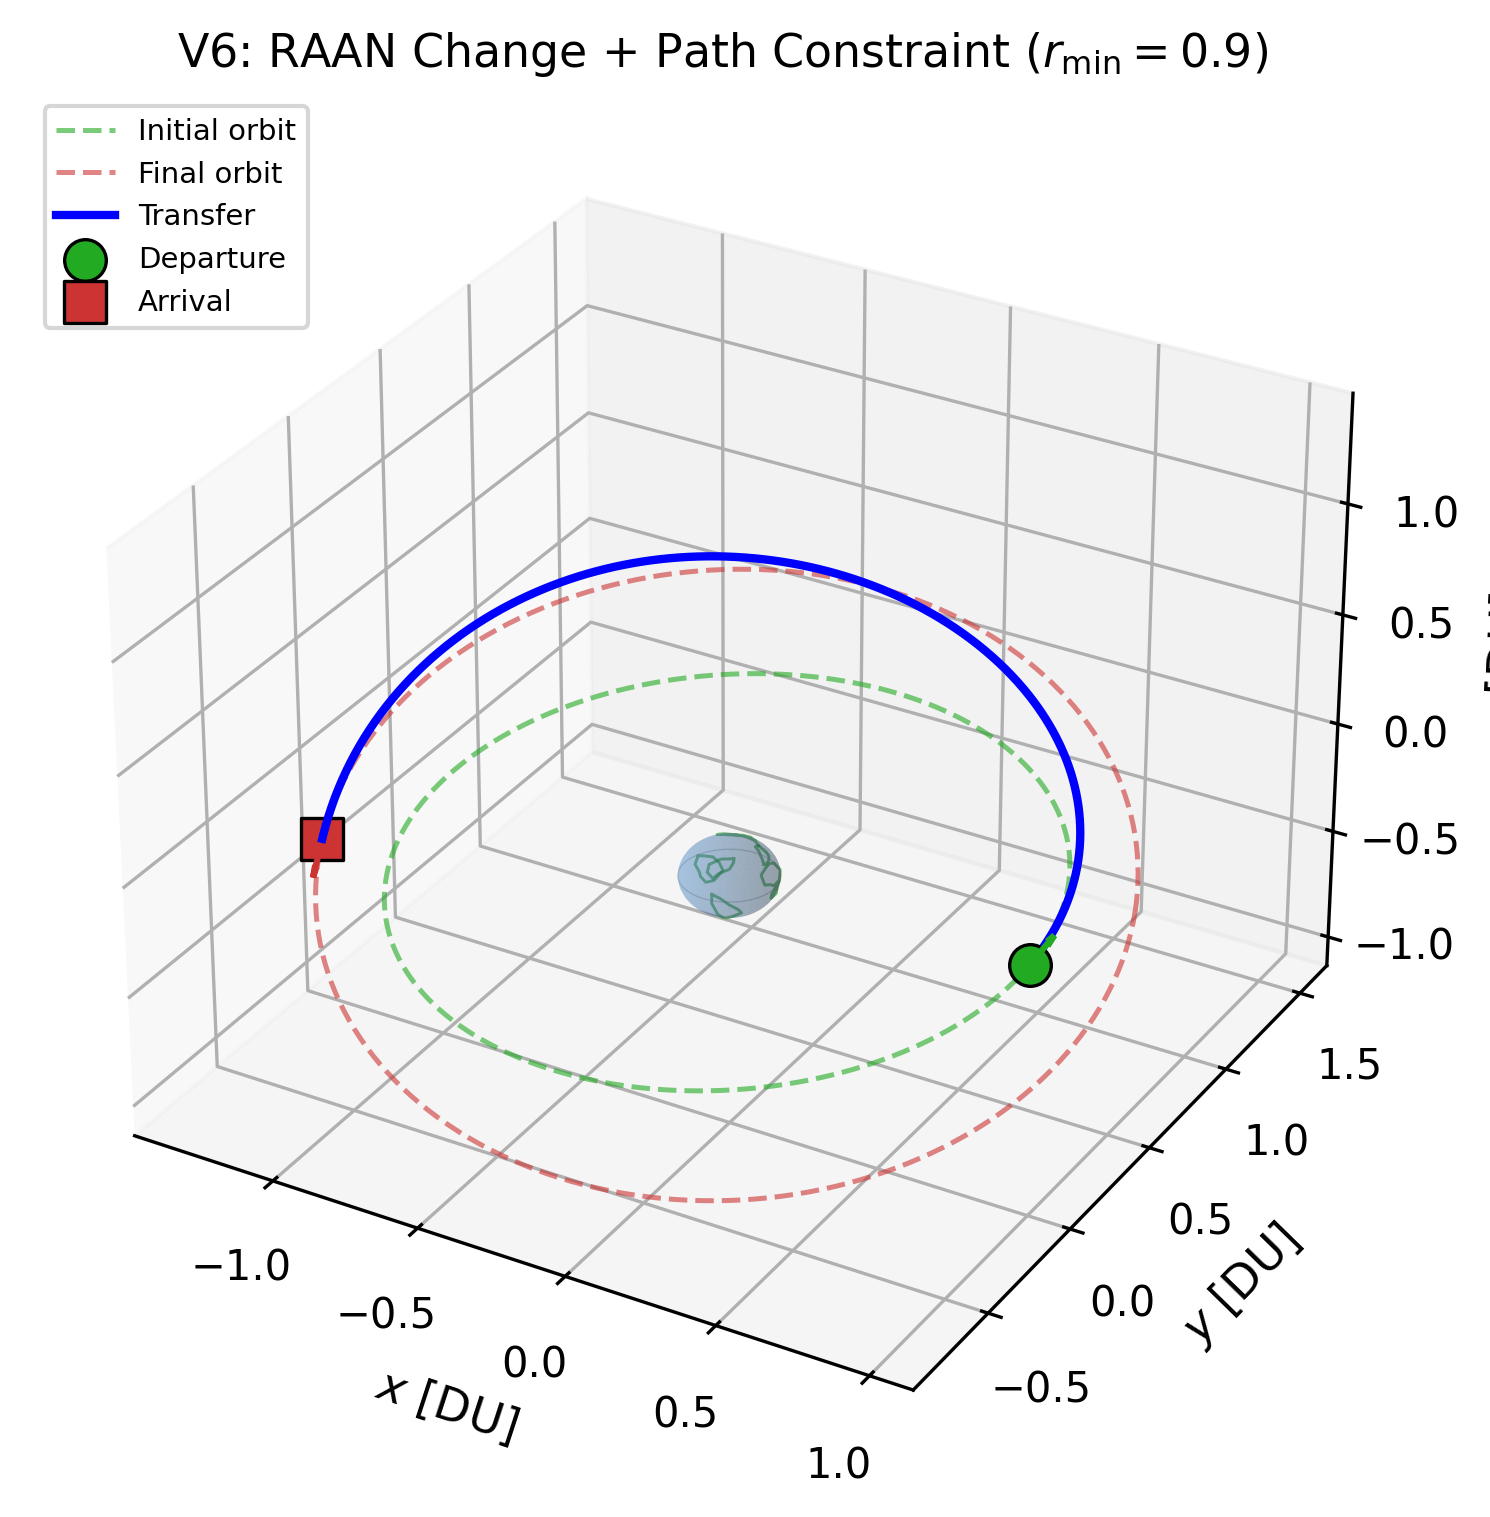
\includegraphics[width=0.75\linewidth]{v6_3d.png}
\caption{V6: RAAN 변경 + 경로 제약 ($r_{\min}=0.9$) 3차원 전이 궤적.}
\label{fig:v6_3d}
\end{figure}

\begin{figure}[htbp]
\centering
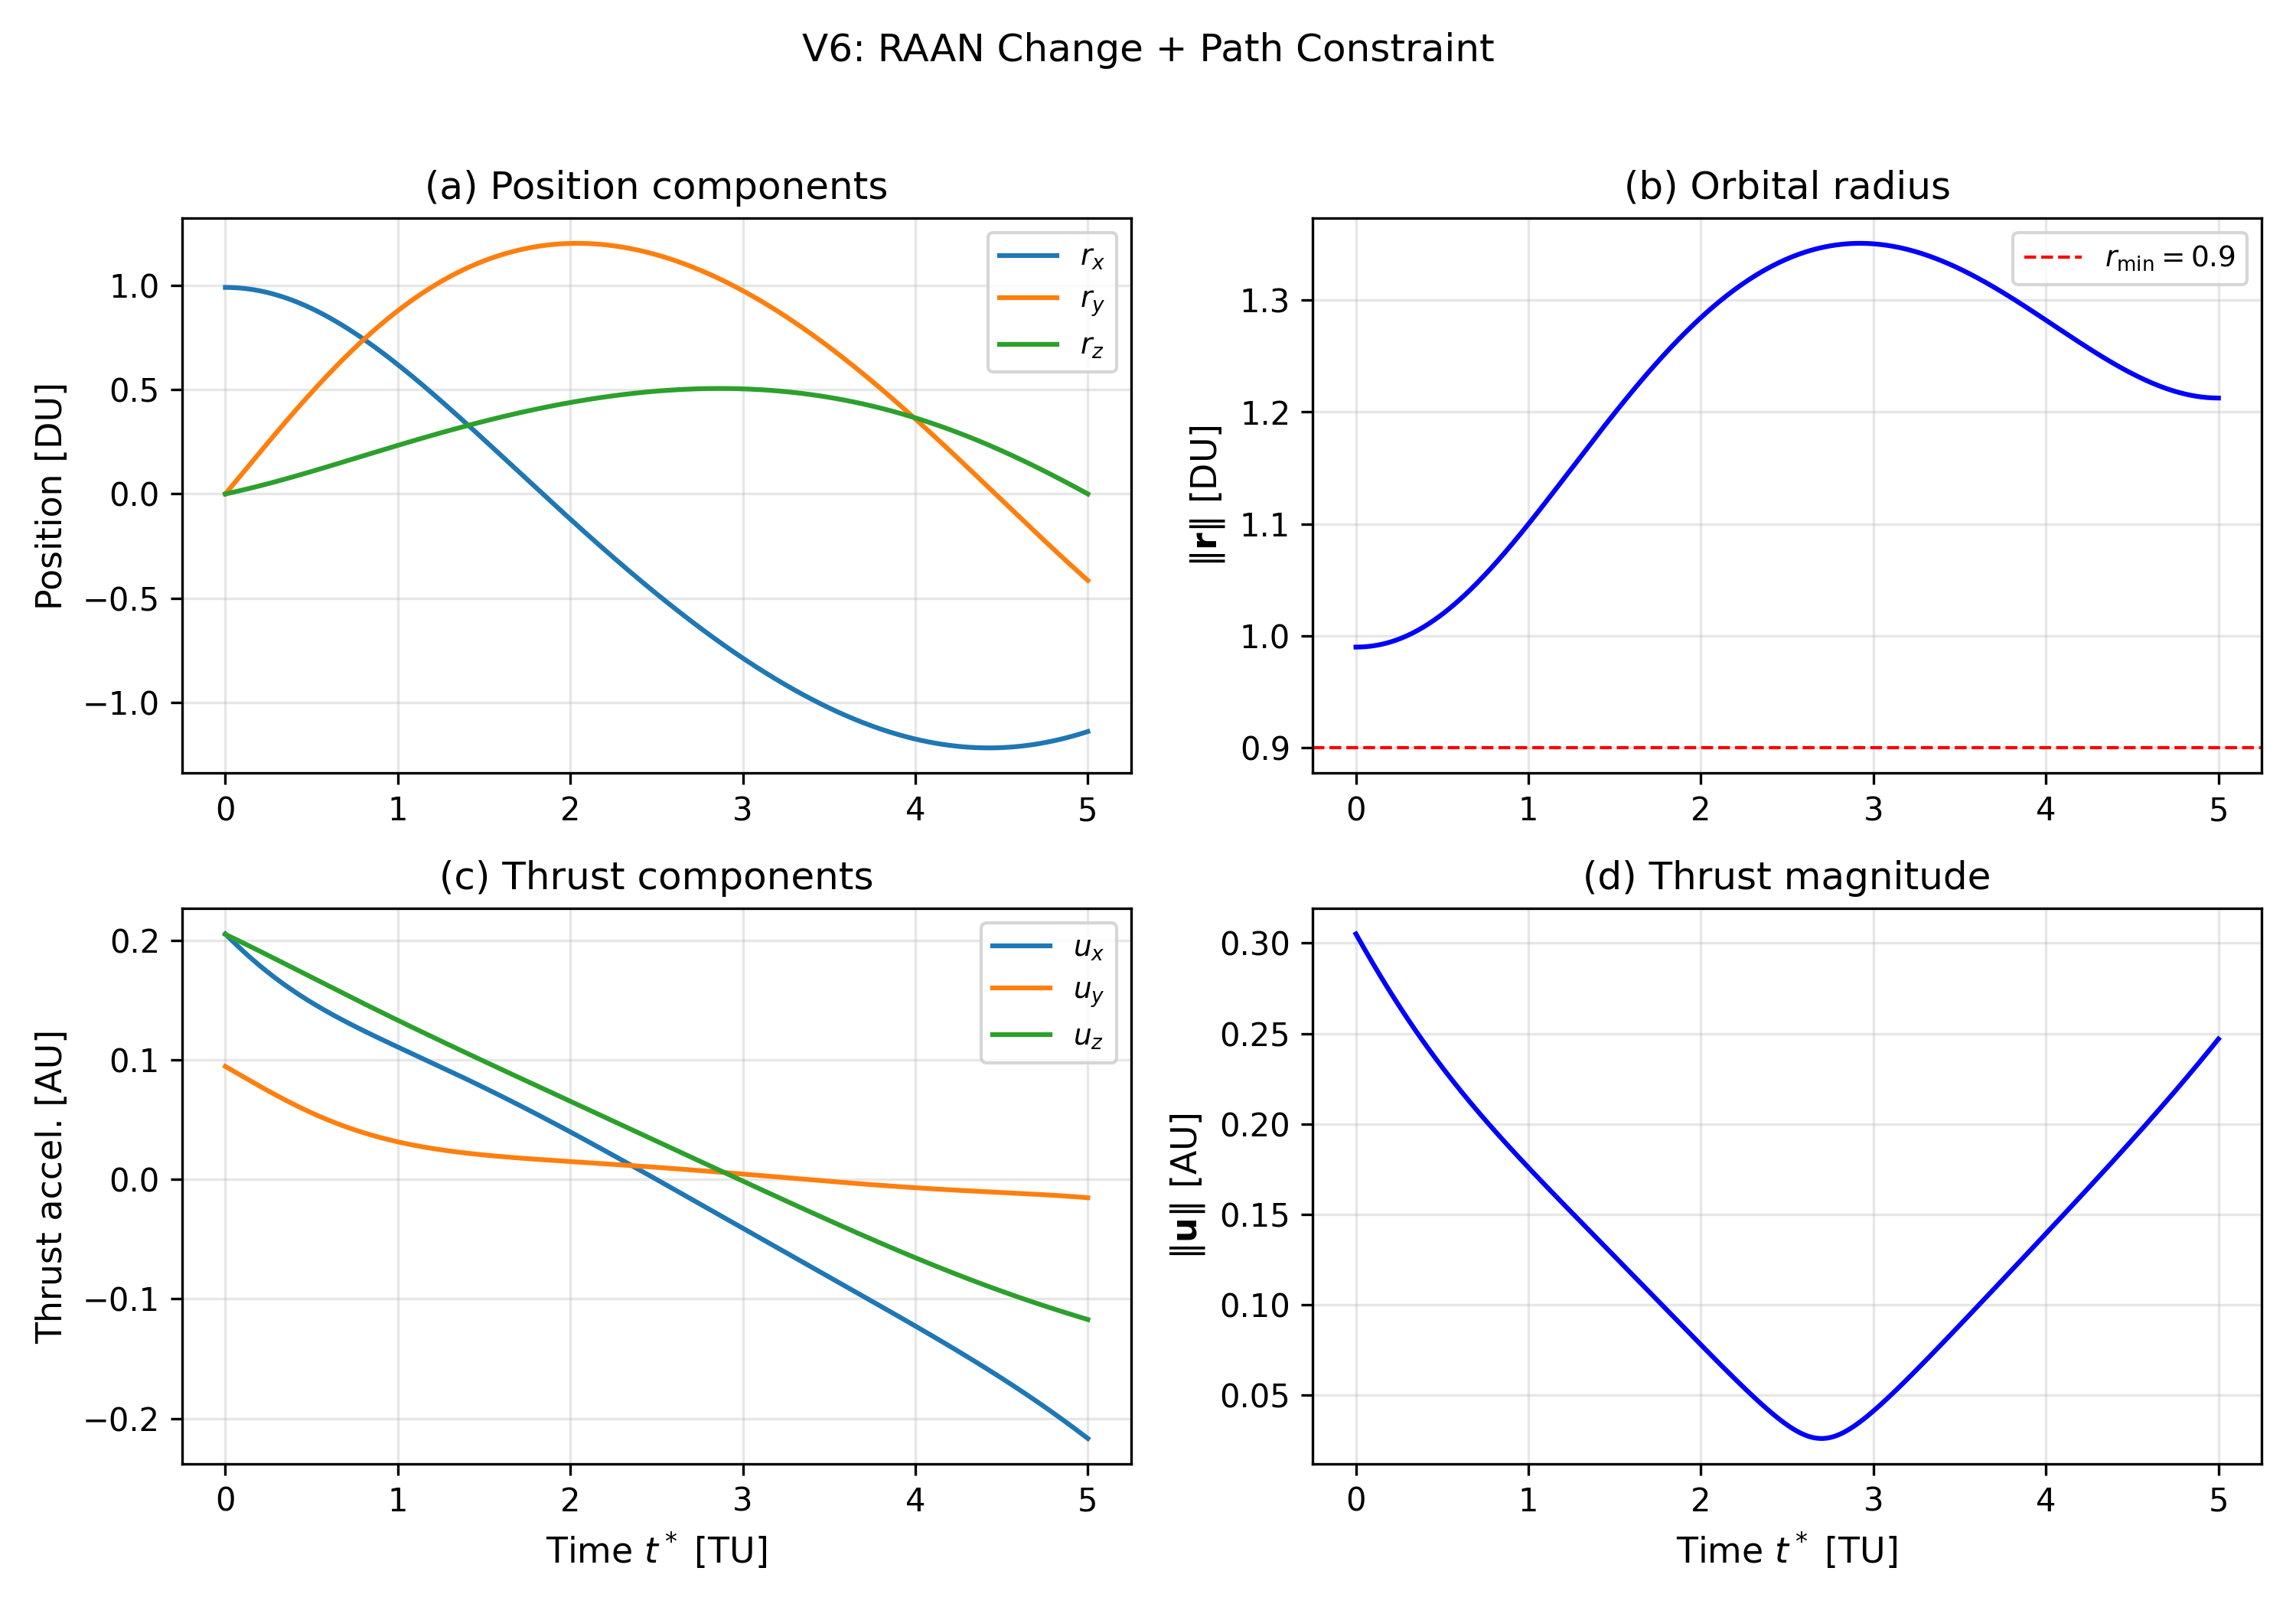
\includegraphics[width=\linewidth]{v6_profiles.png}
\caption{V6: 위치 성분 (a), 궤도 반경 (b), 추력 성분 (c), 추력 크기 (d).
         (b)의 궤도 반경이 $r_{\min}$ 이상을 유지한다.}
\label{fig:v6_profiles}
\end{figure}

\subsection{세분화 구간 수 $K$의 영향}

Table~\ref{tab:K_effect}에 $K = 4, 8, 16$에 대한 결과를 정리하였다.
$K$가 증가하면 제약 수가 늘어나지만 비용과 수렴 특성에는 큰 차이가 없다.
이는 경로 제약이 비활성인 시나리오에서 예상되는 결과이다.

\begin{table}[h]
\centering
\caption{V6 시나리오에서 세분화 구간 수 $K$의 영향.}
\label{tab:K_effect}
\begin{tabular}{rrrrl}
\toprule
$K$ & 제약 수 & 반복 & $J^*$ & BC 위반 \\
\midrule
4  & 60  & 37 & 0.121762 & $5.23 \times 10^{-4}$ \\
8  & 120 & 37 & 0.121761 & $5.28 \times 10^{-4}$ \\
16 & 240 & 34 & 0.121714 & $6.56 \times 10^{-4}$ \\
\bottomrule
\end{tabular}
\end{table}

%% ============================================================
\section{V7: SOCP + 비공면 + 경로 제약}
%% ============================================================

\subsection{시나리오 설정}

세 가지 제약 유형을 동시에 적용하는 통합 테스트이다:
\begin{itemize}
  \item \textbf{경계조건 등식}: 초기/종말 상태 (6개 등식)
  \item \textbf{추력 SOCP}: $\|\mathbf{u}(\tau_j)\| \le u_{\max} = 3.0$
  \item \textbf{경로 부등식}: $\|\mathbf{r}(\tau)\| \ge r_{\min} = 0.9$
\end{itemize}
경사각을 $0^\circ \to 20^\circ$로 변경하면서 반장축을 $1.0 \to 1.2$로 키운다.

\subsection{결과}

34회 반복 후 수렴, BC 위반 $8.69 \times 10^{-4}$,
$J^* = 0.2051$, $\Delta V^* = 1.43$이다.
추력 프로파일의 최댓값은 $\|\mathbf{u}\|_{\max} = 0.377$로,
$u_{\max} = 3.0$에 비해 여유가 있어 추력 제약도 비활성이다.

이 시나리오의 의의는 BC 등식, SOCP 추력, 경로 부등식 세 종류의
제약이 동시에 존재하는 상태에서 솔버가 안정적으로 수렴한다는 것이다.
Fig.~\ref{fig:v7_3d}에 3차원 궤적을,
Fig.~\ref{fig:v7_profiles}에 상태 및 추력 프로파일을 나타내었다.
(d)에서 추력 크기가 $u_{\max}=3.0$ 이하를 유지함을 확인할 수 있다.

\begin{figure}[htbp]
\centering
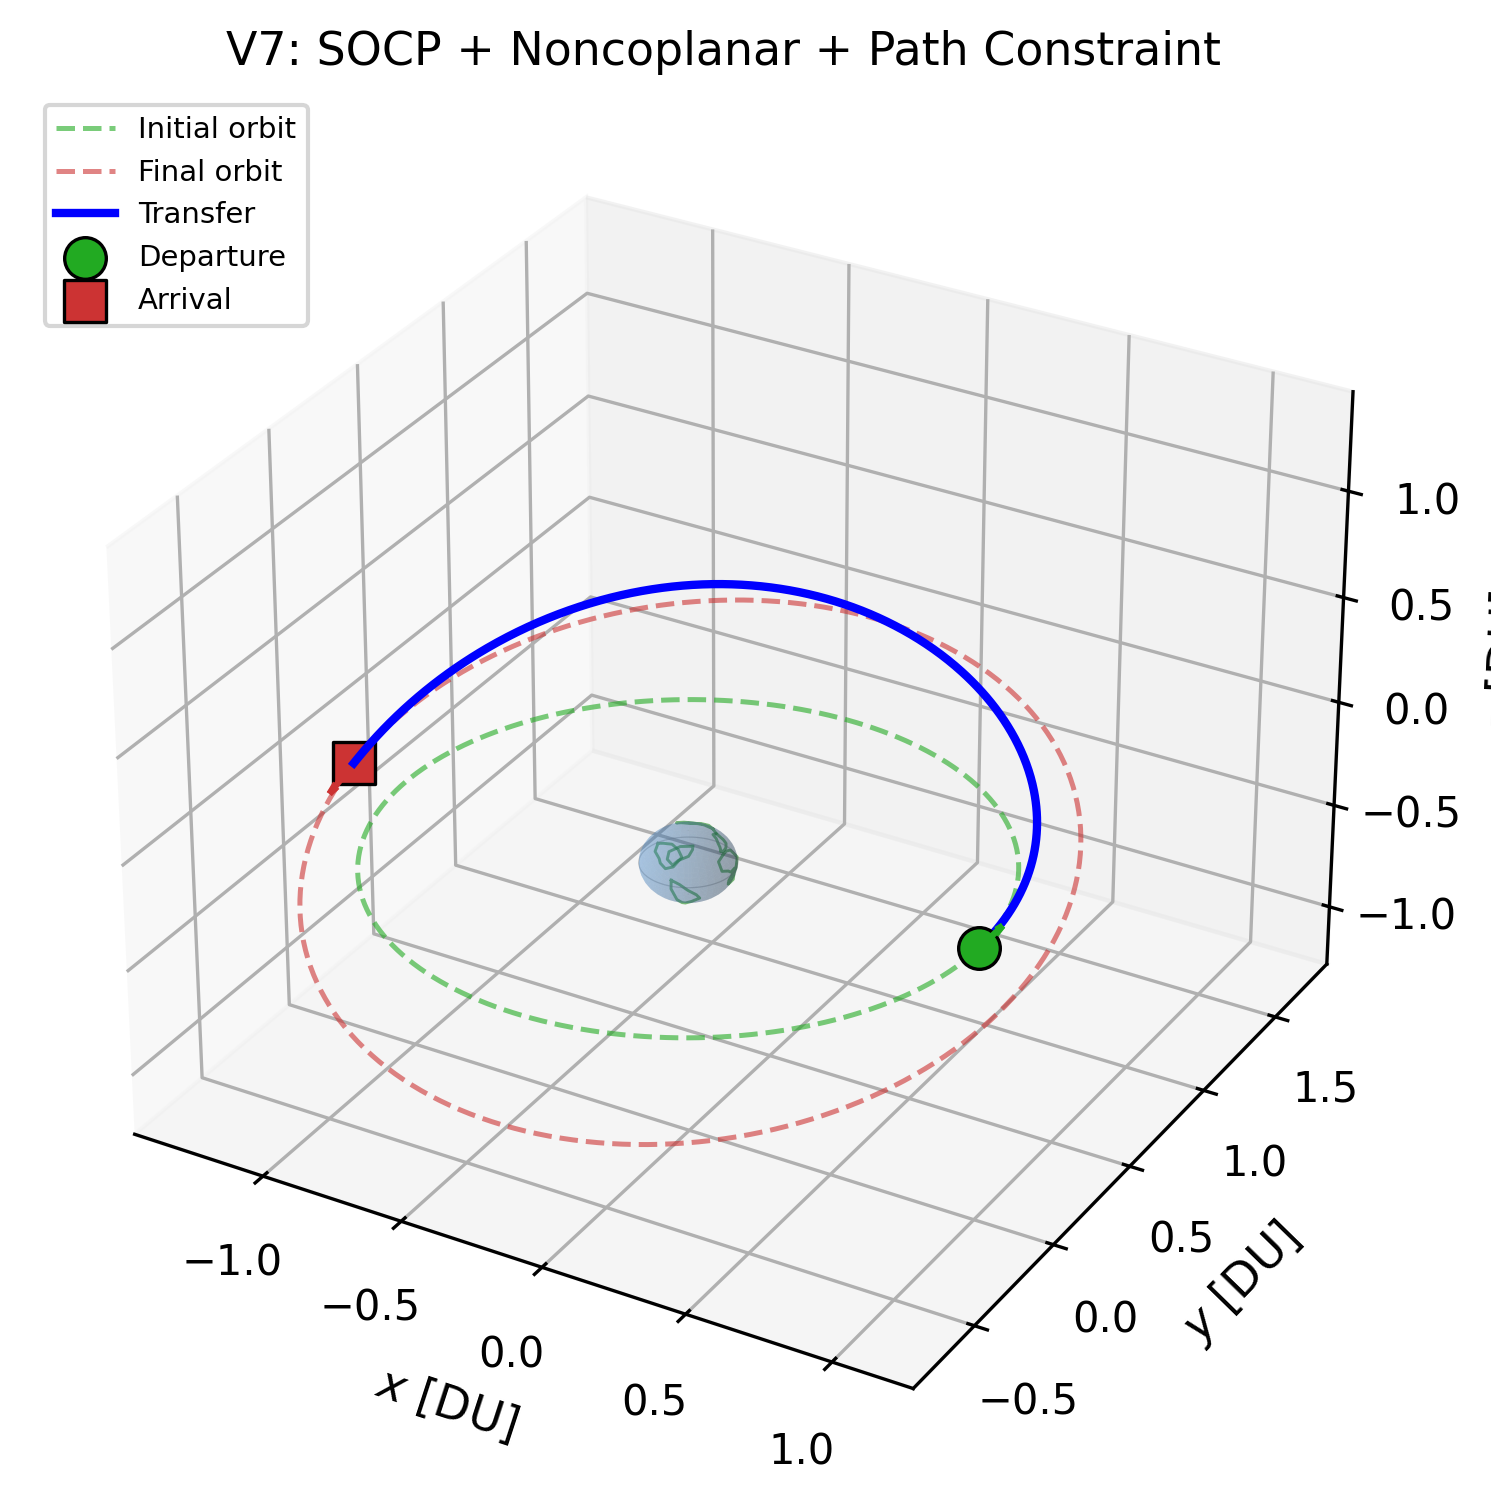
\includegraphics[width=0.75\linewidth]{v7_3d.png}
\caption{V7: SOCP + 비공면 + 경로 제약 3차원 전이 궤적.}
\label{fig:v7_3d}
\end{figure}

\begin{figure}[htbp]
\centering
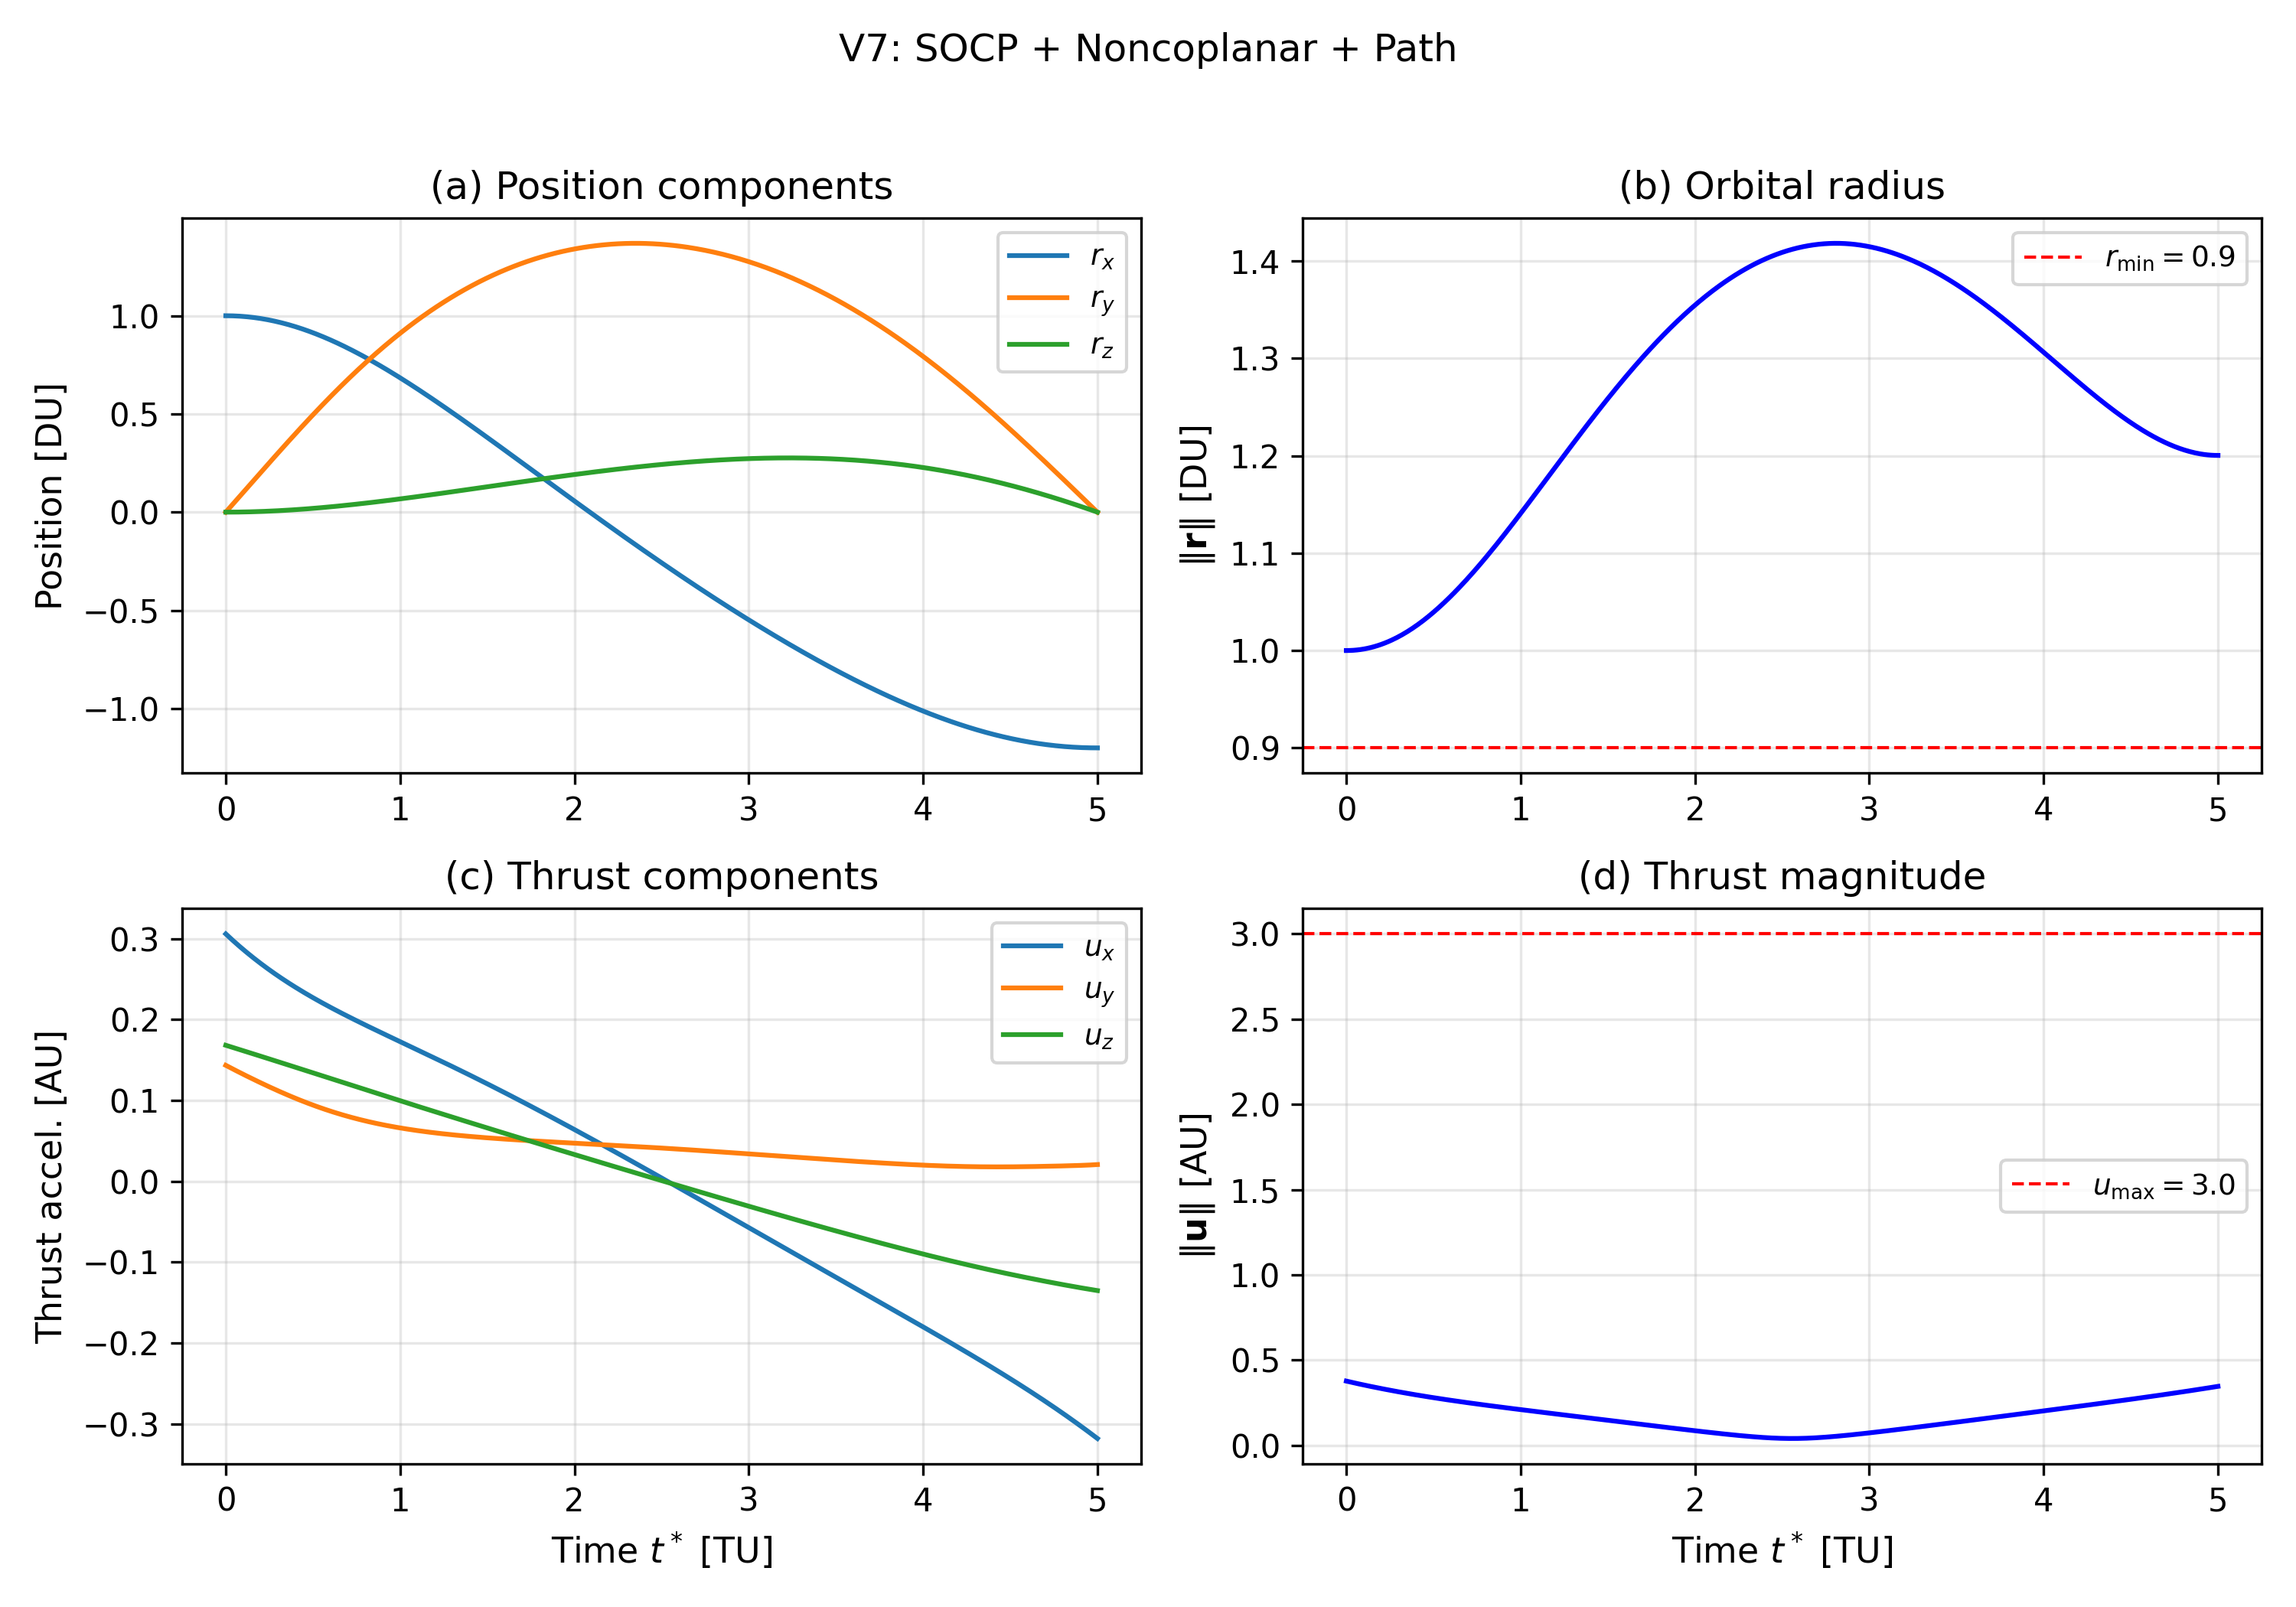
\includegraphics[width=\linewidth]{v7_profiles.png}
\caption{V7: SOCP + 비공면 + 경로 제약 프로파일.
         (b)에 $r_{\min}=0.9$, (d)에 $u_{\max}=3.0$ 제약선을 표시하였다.}
\label{fig:v7_profiles}
\end{figure}

%% ============================================================
\section{수렴 특성 분석}
%% ============================================================

\subsection{비공면 전이의 수렴 특성}

V4--V7 전체에서 SCP는 33--37회 반복으로 수렴하였다.
이는 \cite{report008}의 공면 시나리오(40--42회)와 유사하거나 약간 적은 수치이다.
비공면 전이가 공면보다 수렴이 어렵지 않은 것은,
3차원 동역학의 추가적인 자유도가 오히려 해공간을 넓혀 주기 때문으로 해석된다.
Fig.~\ref{fig:convergence}에 V4--V7의 수렴 곡선을 나타내었다.

\begin{figure}[htbp]
\centering
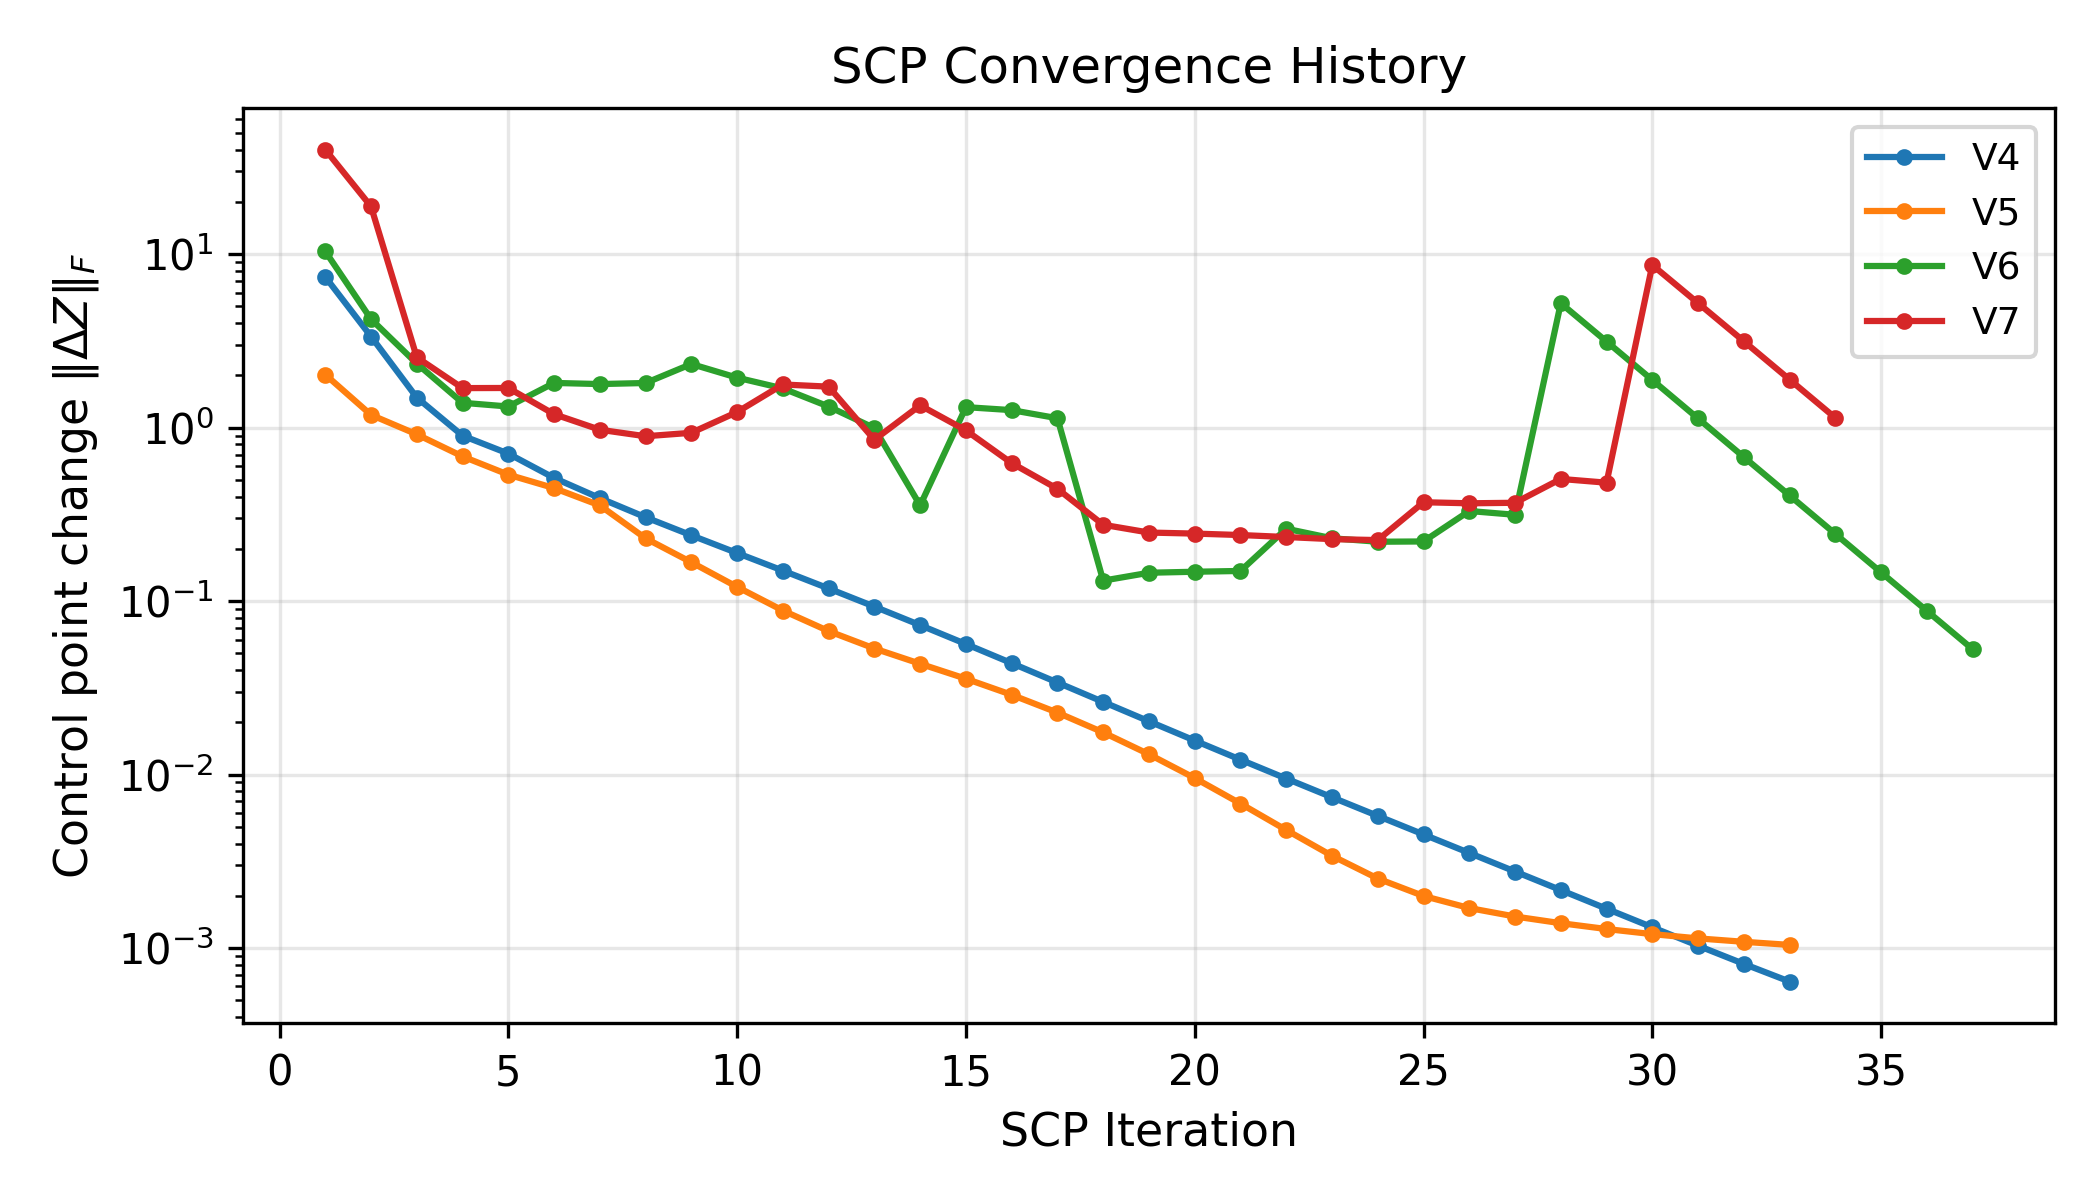
\includegraphics[width=0.85\linewidth]{convergence.png}
\caption{SCP 수렴 이력: 제어점 변화량 $\|\Delta Z\|_F$ (semilog).}
\label{fig:convergence}
\end{figure}

\subsection{RK4 스텝 수의 영향}

반복 중 RK4 적분의 스텝 수 $n_{\mathrm{steps}}$는
드리프트 적분 정밀도에 직접 영향을 미친다.
V4 시나리오에서 스텝 수별 결과를 Table~\ref{tab:nsteps}에 정리하였다.

\begin{table}[h]
\centering
\caption{V4에서 RK4 스텝 수의 영향.}
\label{tab:nsteps}
\begin{tabular}{rrl}
\toprule
$n_{\mathrm{steps}}$ & BC 위반 & 수렴 여부 \\
\midrule
50  & $4.0 \times 10^{-3}$ & 미수렴 \\
200 & $4.3 \times 10^{-4}$ & 수렴 \\
\bottomrule
\end{tabular}
\end{table}

비공면 전이에서는 면외 성분의 정확한 적분이 필요하므로
$n_{\mathrm{steps}} \ge 200$을 권장한다.

%% ============================================================
\section{종합 결과표}
%% ============================================================

\cite{report008}의 V1--V3과 본 노트의 V4--V7을 통합한 결과를
Table~\ref{tab:summary}에 정리하였다.

\begin{table}[h]
\centering
\caption{전체 검증 시나리오 종합 결과.}
\label{tab:summary}
\begin{tabular}{llrlrl}
\toprule
ID & 유형 & 반복 & $J^*$ & $\Delta V^*$ & BC 위반 \\
\midrule
V4 & QP, 경사각 & 33 & 0.2427 & 1.39 & $4.3 \times 10^{-4}$ \\
V5 & QP, 이심률+경사각 & 33 & 0.0864 & 0.93 & $5.4 \times 10^{-4}$ \\
V6 & QP+$r_{\min}$, RAAN & 37 & 0.1218 & 1.10 & $5.3 \times 10^{-4}$ \\
V7 & SOCP+$r_{\min}$, 통합 & 34 & 0.2051 & 1.43 & $8.7 \times 10^{-4}$ \\
\bottomrule
\end{tabular}
\end{table}

%% ============================================================
\section{결론}
%% ============================================================

비공면 3차원 궤도전이에서 베지어--SCP 프레임워크의 수렴을 확인하였다.
주요 발견:
\begin{itemize}
  \item 경사각, RAAN, 이심률의 동시 변경을 포함하는 비공면 전이가
        33--37회 반복으로 안정적으로 수렴한다.
  \item 드 카스텔조 세분화 기반 경로 제약~\cite{report013}이
        SCP 프레임워크에 안정적으로 통합된다.
  \item SOCP 추력 제약, 경로 부등식 제약, BC 등식 제약을
        동시에 적용할 수 있으며 솔버가 안정적이다.
  \item 비공면 전이에서는 RK4 스텝 수를 $\ge 200$으로 설정해야
        드리프트 적분 정밀도가 확보된다.
  \item 대규모 전이($a$ 2배 이상 변경)에서는
        0차 선형화의 한계로 수렴이 어려울 수 있으며,
        1차 SCP(상태 천이 행렬 활용)나 커플링 행렬~\cite{report012}의
        통합이 향후 과제이다.
\end{itemize}

%% ============================================================
\bibliographystyle{IEEEtran}
\bibliography{references}

\end{document}
